%%===========================================================%%
%%                                                           %%
%%                   DE/DX ADJUSTMENT APPENDIX               %%
%%                                                           %%
%%===========================================================%%

\chapter{TPC track reconstruction efficiency}\label{appendix:tpcEff}


%---------------------------
\begin{figure}[hb]
\caption[TPC acceptance and reconstruction efficiency of $\pi^{-}$ for runs with dead sector \#19.]{TPC acceptance and reconstruction efficiency of $\pi^{-}$ for runs with dead sector \#19. Each plot represents the TPC efficiency $\epsilon_{\text{TPC}}$ ($z$-axis) as a function of true particle pseudorapidity $\eta$ ($x$-axis) and transverse momentum $p_{T}$ ($y$-axis) in single $z$-vertex bin whose range is given at the top. Red lines and arrows indicate region accepted in analyses.}\label{fig:tpcEff_pion_minus}
\centering
\parbox{0.495\textwidth}{
  \centering
  \includegraphics[width=\linewidth,page=3]{graphics/eff/Eff2D_TPC_pion_Minus_RunRange1.pdf}\\
  \includegraphics[width=\linewidth,page=5]{graphics/eff/Eff2D_TPC_pion_Minus_RunRange1.pdf}\\
  \includegraphics[width=\linewidth,page=7]{graphics/eff/Eff2D_TPC_pion_Minus_RunRange1.pdf}\\
  \includegraphics[width=\linewidth,page=9]{graphics/eff/Eff2D_TPC_pion_Minus_RunRange1.pdf}
}~
\parbox{0.495\textwidth}{
  \centering
  \includegraphics[width=\linewidth,page=4]{graphics/eff/Eff2D_TPC_pion_Minus_RunRange1.pdf}\\
  \includegraphics[width=\linewidth,page=6]{graphics/eff/Eff2D_TPC_pion_Minus_RunRange1.pdf}\\
  \includegraphics[width=\linewidth,page=8]{graphics/eff/Eff2D_TPC_pion_Minus_RunRange1.pdf}\\
  \includegraphics[width=\linewidth,page=10]{graphics/eff/Eff2D_TPC_pion_Minus_RunRange1.pdf}
}%
\end{figure}
\begin{figure}[hb]\ContinuedFloat
% ~\\[32pt]
\centering
\parbox{0.495\textwidth}{
  \centering
  \includegraphics[width=\linewidth,page=11]{graphics/eff/Eff2D_TPC_pion_Minus_RunRange1.pdf}\\
  \includegraphics[width=\linewidth,page=13]{graphics/eff/Eff2D_TPC_pion_Minus_RunRange1.pdf}\\
  \includegraphics[width=\linewidth,page=15]{graphics/eff/Eff2D_TPC_pion_Minus_RunRange1.pdf}\\
  \includegraphics[width=\linewidth,page=17]{graphics/eff/Eff2D_TPC_pion_Minus_RunRange1.pdf}
}~
\parbox{0.495\textwidth}{
  \centering
  \includegraphics[width=\linewidth,page=12]{graphics/eff/Eff2D_TPC_pion_Minus_RunRange1.pdf}\\
  \includegraphics[width=\linewidth,page=14]{graphics/eff/Eff2D_TPC_pion_Minus_RunRange1.pdf}\\
  \includegraphics[width=\linewidth,page=16]{graphics/eff/Eff2D_TPC_pion_Minus_RunRange1.pdf}\\
  \includegraphics[width=\linewidth,page=18]{graphics/eff/Eff2D_TPC_pion_Minus_RunRange1.pdf}
}%
\end{figure}
%---------------------------

%---------------------------
\begin{figure}[hb]
	\caption[TPC acceptance and reconstruction efficiency of $\pi^{-}$ for runs with  sector \#19 back in operation.]{TPC acceptance and reconstruction efficiency of $\pi^{-}$ for runs with  sector \#19 back in operation. Each plot represents the TPC efficiency $\epsilon_{\text{TPC}}$ ($z$-axis) as a function of true particle pseudorapidity $\eta$ ($x$-axis) and transverse momentum $p_{T}$ ($y$-axis) in single $z$-vertex bin whose range is given at the top. Red lines and arrows indicate region accepted in analyses.}\label{fig:tpcEff_pion_minus1}
	\centering
	\parbox{0.495\textwidth}{
		\centering
		\includegraphics[width=\linewidth,page=3]{graphics/eff/Eff2D_TPC_pion_Minus_RunRange2.pdf}\\
		\includegraphics[width=\linewidth,page=5]{graphics/eff/Eff2D_TPC_pion_Minus_RunRange2.pdf}\\
		\includegraphics[width=\linewidth,page=7]{graphics/eff/Eff2D_TPC_pion_Minus_RunRange2.pdf}\\
		\includegraphics[width=\linewidth,page=9]{graphics/eff/Eff2D_TPC_pion_Minus_RunRange2.pdf}
	}~
	\parbox{0.495\textwidth}{
		\centering
		\includegraphics[width=\linewidth,page=4]{graphics/eff/Eff2D_TPC_pion_Minus_RunRange2.pdf}\\
		\includegraphics[width=\linewidth,page=6]{graphics/eff/Eff2D_TPC_pion_Minus_RunRange2.pdf}\\
		\includegraphics[width=\linewidth,page=8]{graphics/eff/Eff2D_TPC_pion_Minus_RunRange2.pdf}\\
		\includegraphics[width=\linewidth,page=10]{graphics/eff/Eff2D_TPC_pion_Minus_RunRange2.pdf}
	}%
\end{figure}
\begin{figure}[hb]\ContinuedFloat
	% ~\\[32pt]
	\centering
	\parbox{0.495\textwidth}{
		\centering
		\includegraphics[width=\linewidth,page=11]{graphics/eff/Eff2D_TPC_pion_Minus_RunRange2.pdf}\\
		\includegraphics[width=\linewidth,page=13]{graphics/eff/Eff2D_TPC_pion_Minus_RunRange2.pdf}\\
		\includegraphics[width=\linewidth,page=15]{graphics/eff/Eff2D_TPC_pion_Minus_RunRange2.pdf}\\
		\includegraphics[width=\linewidth,page=17]{graphics/eff/Eff2D_TPC_pion_Minus_RunRange2.pdf}
	}~
	\parbox{0.495\textwidth}{
		\centering
		\includegraphics[width=\linewidth,page=12]{graphics/eff/Eff2D_TPC_pion_Minus_RunRange2.pdf}\\
		\includegraphics[width=\linewidth,page=14]{graphics/eff/Eff2D_TPC_pion_Minus_RunRange2.pdf}\\
		\includegraphics[width=\linewidth,page=16]{graphics/eff/Eff2D_TPC_pion_Minus_RunRange2.pdf}\\
		\includegraphics[width=\linewidth,page=18]{graphics/eff/Eff2D_TPC_pion_Minus_RunRange2.pdf}
	}%
\end{figure}
%---------------------------

%---------------------------
\begin{figure}[hb]
\caption[TPC acceptance and reconstruction efficiency of $\pi^{+}$ for runs with dead sector \#19.]{TPC acceptance and reconstruction efficiency of $\pi^{+}$ for runs with dead sector \#19. Each plot represents the TPC efficiency $\epsilon_{\text{TPC}}$ ($z$-axis) as a function of true particle pseudorapidity $\eta$ ($x$-axis) and transverse momentum $p_{T}$ ($y$-axis) in single $z$-vertex bin whose range is given at the top. Red lines and arrows indicate region accepted in analyses.}\label{fig:tpcEff_pion_plus}
\centering
\parbox{0.495\textwidth}{
  \centering
  \includegraphics[width=\linewidth,page=3]{graphics/eff/Eff2D_TPC_pion_Plus_RunRange1.pdf}\\
  \includegraphics[width=\linewidth,page=5]{graphics/eff/Eff2D_TPC_pion_Plus_RunRange1.pdf}\\
  \includegraphics[width=\linewidth,page=7]{graphics/eff/Eff2D_TPC_pion_Plus_RunRange1.pdf}\\
  \includegraphics[width=\linewidth,page=9]{graphics/eff/Eff2D_TPC_pion_Plus_RunRange1.pdf}
}~
\parbox{0.495\textwidth}{
  \centering
  \includegraphics[width=\linewidth,page=4]{graphics/eff/Eff2D_TPC_pion_Plus_RunRange1.pdf}\\
  \includegraphics[width=\linewidth,page=6]{graphics/eff/Eff2D_TPC_pion_Plus_RunRange1.pdf}\\
  \includegraphics[width=\linewidth,page=8]{graphics/eff/Eff2D_TPC_pion_Plus_RunRange1.pdf}\\
  \includegraphics[width=\linewidth,page=10]{graphics/eff/Eff2D_TPC_pion_Plus_RunRange1.pdf}
}%
\end{figure}
\begin{figure}[hb]\ContinuedFloat
% ~\\[32pt]
\centering
\parbox{0.495\textwidth}{
  \centering
  \includegraphics[width=\linewidth,page=11]{graphics/eff/Eff2D_TPC_pion_Plus_RunRange1.pdf}\\
  \includegraphics[width=\linewidth,page=13]{graphics/eff/Eff2D_TPC_pion_Plus_RunRange1.pdf}\\
  \includegraphics[width=\linewidth,page=15]{graphics/eff/Eff2D_TPC_pion_Plus_RunRange1.pdf}\\
  \includegraphics[width=\linewidth,page=17]{graphics/eff/Eff2D_TPC_pion_Plus_RunRange1.pdf}
}~
\parbox{0.495\textwidth}{
  \centering
  \includegraphics[width=\linewidth,page=12]{graphics/eff/Eff2D_TPC_pion_Plus_RunRange1.pdf}\\
  \includegraphics[width=\linewidth,page=14]{graphics/eff/Eff2D_TPC_pion_Plus_RunRange1.pdf}\\
  \includegraphics[width=\linewidth,page=16]{graphics/eff/Eff2D_TPC_pion_Plus_RunRange1.pdf}\\
  \includegraphics[width=\linewidth,page=18]{graphics/eff/Eff2D_TPC_pion_Plus_RunRange1.pdf}
}%
\end{figure}
%---------------------------


%---------------------------
\begin{figure}[hb]
	\caption[TPC acceptance and reconstruction efficiency of $\pi^{+}$ for runs with  sector \#19 back in operation.]{TPC acceptance and reconstruction efficiency of $\pi^{+}$ for runs with  sector \#19 back in operation. Each plot represents the TPC efficiency $\epsilon_{\text{TPC}}$ ($z$-axis) as a function of true particle pseudorapidity $\eta$ ($x$-axis) and transverse momentum $p_{T}$ ($y$-axis) in single $z$-vertex bin whose range is given at the top. Red lines and arrows indicate region accepted in analyses.}\label{fig:tpcEff_pion_plus1}
	\centering
	\parbox{0.495\textwidth}{
		\centering
		\includegraphics[width=\linewidth,page=3]{graphics/eff/Eff2D_TPC_pion_Plus_RunRange2.pdf}\\
		\includegraphics[width=\linewidth,page=5]{graphics/eff/Eff2D_TPC_pion_Plus_RunRange2.pdf}\\
		\includegraphics[width=\linewidth,page=7]{graphics/eff/Eff2D_TPC_pion_Plus_RunRange2.pdf}\\
		\includegraphics[width=\linewidth,page=9]{graphics/eff/Eff2D_TPC_pion_Plus_RunRange2.pdf}
	}~
	\parbox{0.495\textwidth}{
		\centering
		\includegraphics[width=\linewidth,page=4]{graphics/eff/Eff2D_TPC_pion_Plus_RunRange2.pdf}\\
		\includegraphics[width=\linewidth,page=6]{graphics/eff/Eff2D_TPC_pion_Plus_RunRange2.pdf}\\
		\includegraphics[width=\linewidth,page=8]{graphics/eff/Eff2D_TPC_pion_Plus_RunRange2.pdf}\\
		\includegraphics[width=\linewidth,page=10]{graphics/eff/Eff2D_TPC_pion_Plus_RunRange2.pdf}
	}%
\end{figure}
\begin{figure}[hb]\ContinuedFloat
	% ~\\[32pt]
	\centering
	\parbox{0.495\textwidth}{
		\centering
		\includegraphics[width=\linewidth,page=11]{graphics/eff/Eff2D_TPC_pion_Plus_RunRange2.pdf}\\
		\includegraphics[width=\linewidth,page=13]{graphics/eff/Eff2D_TPC_pion_Plus_RunRange2.pdf}\\
		\includegraphics[width=\linewidth,page=15]{graphics/eff/Eff2D_TPC_pion_Plus_RunRange2.pdf}\\
		\includegraphics[width=\linewidth,page=17]{graphics/eff/Eff2D_TPC_pion_Plus_RunRange2.pdf}
	}~
	\parbox{0.495\textwidth}{
		\centering
		\includegraphics[width=\linewidth,page=12]{graphics/eff/Eff2D_TPC_pion_Plus_RunRange2.pdf}\\
		\includegraphics[width=\linewidth,page=14]{graphics/eff/Eff2D_TPC_pion_Plus_RunRange2.pdf}\\
		\includegraphics[width=\linewidth,page=16]{graphics/eff/Eff2D_TPC_pion_Plus_RunRange2.pdf}\\
		\includegraphics[width=\linewidth,page=18]{graphics/eff/Eff2D_TPC_pion_Plus_RunRange2.pdf}
	}%
\end{figure}
%---------------------------


%---------------------------
\begin{figure}[hb]
\caption[TPC acceptance and reconstruction efficiency of $K^{-}$ for runs with dead sector \#19.]{TPC acceptance and reconstruction efficiency of $K^{-}$ for runs with dead sector \#19. Each plot represents the TPC efficiency $\epsilon_{\text{TPC}}$ ($z$-axis) as a function of true particle pseudorapidity $\eta$ ($x$-axis) and transverse momentum $p_{T}$ ($y$-axis) in single $z$-vertex bin whose range is given at the top. Red lines and arrows indicate region accepted in analyses.}\label{fig:tpcEff_kaon_minus}
\centering
\parbox{0.495\textwidth}{
  \centering
  \includegraphics[width=\linewidth,page=3]{graphics/eff/Eff2D_TPC_kaon_Minus_RunRange1.pdf}\\
  \includegraphics[width=\linewidth,page=5]{graphics/eff/Eff2D_TPC_kaon_Minus_RunRange1.pdf}\\
  \includegraphics[width=\linewidth,page=7]{graphics/eff/Eff2D_TPC_kaon_Minus_RunRange1.pdf}\\
  \includegraphics[width=\linewidth,page=9]{graphics/eff/Eff2D_TPC_kaon_Minus_RunRange1.pdf}
}~
\parbox{0.495\textwidth}{
  \centering
  \includegraphics[width=\linewidth,page=4]{graphics/eff/Eff2D_TPC_kaon_Minus_RunRange1.pdf}\\
  \includegraphics[width=\linewidth,page=6]{graphics/eff/Eff2D_TPC_kaon_Minus_RunRange1.pdf}\\
  \includegraphics[width=\linewidth,page=8]{graphics/eff/Eff2D_TPC_kaon_Minus_RunRange1.pdf}\\
  \includegraphics[width=\linewidth,page=10]{graphics/eff/Eff2D_TPC_kaon_Minus_RunRange1.pdf}
}%
\end{figure}
\begin{figure}[hb]\ContinuedFloat
% ~\\[32pt]
\centering
\parbox{0.495\textwidth}{
  \centering
  \includegraphics[width=\linewidth,page=11]{graphics/eff/Eff2D_TPC_kaon_Minus_RunRange1.pdf}\\
  \includegraphics[width=\linewidth,page=13]{graphics/eff/Eff2D_TPC_kaon_Minus_RunRange1.pdf}\\
  \includegraphics[width=\linewidth,page=15]{graphics/eff/Eff2D_TPC_kaon_Minus_RunRange1.pdf}\\
  \includegraphics[width=\linewidth,page=17]{graphics/eff/Eff2D_TPC_kaon_Minus_RunRange1.pdf}
}~
\parbox{0.495\textwidth}{
  \centering
  \includegraphics[width=\linewidth,page=12]{graphics/eff/Eff2D_TPC_kaon_Minus_RunRange1.pdf}\\
  \includegraphics[width=\linewidth,page=14]{graphics/eff/Eff2D_TPC_kaon_Minus_RunRange1.pdf}\\
  \includegraphics[width=\linewidth,page=16]{graphics/eff/Eff2D_TPC_kaon_Minus_RunRange1.pdf}\\
  \includegraphics[width=\linewidth,page=18]{graphics/eff/Eff2D_TPC_kaon_Minus_RunRange1.pdf}
}%
\end{figure}
%---------------------------

%---------------------------
\begin{figure}[hb]
	\caption[TPC acceptance and reconstruction efficiency of $K^{-}$ for runs with sector \#19 back in operation.]{TPC acceptance and reconstruction efficiency of $K^{-}$ for runs with sector \#19 back in operation. Each plot represents the TPC efficiency $\epsilon_{\text{TPC}}$ ($z$-axis) as a function of true particle pseudorapidity $\eta$ ($x$-axis) and transverse momentum $p_{T}$ ($y$-axis) in single $z$-vertex bin whose range is given at the top. Red lines and arrows indicate region accepted in analyses.}\label{fig:tpcEff_kaon_minus1}
	\centering
	\parbox{0.495\textwidth}{
		\centering
		\includegraphics[width=\linewidth,page=3]{graphics/eff/Eff2D_TPC_kaon_Minus_RunRange2.pdf}\\
		\includegraphics[width=\linewidth,page=5]{graphics/eff/Eff2D_TPC_kaon_Minus_RunRange2.pdf}\\
		\includegraphics[width=\linewidth,page=7]{graphics/eff/Eff2D_TPC_kaon_Minus_RunRange2.pdf}\\
		\includegraphics[width=\linewidth,page=9]{graphics/eff/Eff2D_TPC_kaon_Minus_RunRange2.pdf}
	}~
	\parbox{0.495\textwidth}{
		\centering
		\includegraphics[width=\linewidth,page=4]{graphics/eff/Eff2D_TPC_kaon_Minus_RunRange2.pdf}\\
		\includegraphics[width=\linewidth,page=6]{graphics/eff/Eff2D_TPC_kaon_Minus_RunRange2.pdf}\\
		\includegraphics[width=\linewidth,page=8]{graphics/eff/Eff2D_TPC_kaon_Minus_RunRange2.pdf}\\
		\includegraphics[width=\linewidth,page=10]{graphics/eff/Eff2D_TPC_kaon_Minus_RunRange2.pdf}
	}%
\end{figure}
\begin{figure}[hb]\ContinuedFloat
	% ~\\[32pt]
	\centering
	\parbox{0.495\textwidth}{
		\centering
		\includegraphics[width=\linewidth,page=11]{graphics/eff/Eff2D_TPC_kaon_Minus_RunRange2.pdf}\\
		\includegraphics[width=\linewidth,page=13]{graphics/eff/Eff2D_TPC_kaon_Minus_RunRange2.pdf}\\
		\includegraphics[width=\linewidth,page=15]{graphics/eff/Eff2D_TPC_kaon_Minus_RunRange2.pdf}\\
		\includegraphics[width=\linewidth,page=17]{graphics/eff/Eff2D_TPC_kaon_Minus_RunRange2.pdf}
	}~
	\parbox{0.495\textwidth}{
		\centering
		\includegraphics[width=\linewidth,page=12]{graphics/eff/Eff2D_TPC_kaon_Minus_RunRange2.pdf}\\
		\includegraphics[width=\linewidth,page=14]{graphics/eff/Eff2D_TPC_kaon_Minus_RunRange2.pdf}\\
		\includegraphics[width=\linewidth,page=16]{graphics/eff/Eff2D_TPC_kaon_Minus_RunRange2.pdf}\\
		\includegraphics[width=\linewidth,page=18]{graphics/eff/Eff2D_TPC_kaon_Minus_RunRange2.pdf}
	}%
\end{figure}
%---------------------------


%---------------------------
\begin{figure}[hb]
\caption[TPC acceptance and reconstruction efficiency of $K^{+}$ for runs with dead sector \#19.]{TPC acceptance and reconstruction efficiency of $K^{+}$ for runs with dead sector \#19. Each plot represents the TPC efficiency $\epsilon_{\text{TPC}}$ ($z$-axis) as a function of true particle pseudorapidity $\eta$ ($x$-axis) and transverse momentum $p_{T}$ ($y$-axis) in single $z$-vertex bin whose range is given at the top. Red lines and arrows indicate region accepted in analyses.}\label{fig:tpcEff_kaon_plus}
\centering
\parbox{0.495\textwidth}{
  \centering
  \includegraphics[width=\linewidth,page=3]{graphics/eff/Eff2D_TPC_kaon_Plus_RunRange1.pdf}\\
  \includegraphics[width=\linewidth,page=5]{graphics/eff/Eff2D_TPC_kaon_Plus_RunRange1.pdf}\\
  \includegraphics[width=\linewidth,page=7]{graphics/eff/Eff2D_TPC_kaon_Plus_RunRange1.pdf}\\
  \includegraphics[width=\linewidth,page=9]{graphics/eff/Eff2D_TPC_kaon_Plus_RunRange1.pdf}
}~
\parbox{0.495\textwidth}{
  \centering
  \includegraphics[width=\linewidth,page=4]{graphics/eff/Eff2D_TPC_kaon_Plus_RunRange1.pdf}\\
  \includegraphics[width=\linewidth,page=6]{graphics/eff/Eff2D_TPC_kaon_Plus_RunRange1.pdf}\\
  \includegraphics[width=\linewidth,page=8]{graphics/eff/Eff2D_TPC_kaon_Plus_RunRange1.pdf}\\
  \includegraphics[width=\linewidth,page=10]{graphics/eff/Eff2D_TPC_kaon_Plus_RunRange1.pdf}
}%
\end{figure}
\begin{figure}[hb]\ContinuedFloat
% ~\\[32pt]
\centering
\parbox{0.495\textwidth}{
  \centering
  \includegraphics[width=\linewidth,page=11]{graphics/eff/Eff2D_TPC_kaon_Plus_RunRange1.pdf}\\
  \includegraphics[width=\linewidth,page=13]{graphics/eff/Eff2D_TPC_kaon_Plus_RunRange1.pdf}\\
  \includegraphics[width=\linewidth,page=15]{graphics/eff/Eff2D_TPC_kaon_Plus_RunRange1.pdf}\\
  \includegraphics[width=\linewidth,page=17]{graphics/eff/Eff2D_TPC_kaon_Plus_RunRange1.pdf}
}~
\parbox{0.495\textwidth}{
  \centering
  \includegraphics[width=\linewidth,page=12]{graphics/eff/Eff2D_TPC_kaon_Plus_RunRange1.pdf}\\
  \includegraphics[width=\linewidth,page=14]{graphics/eff/Eff2D_TPC_kaon_Plus_RunRange1.pdf}\\
  \includegraphics[width=\linewidth,page=16]{graphics/eff/Eff2D_TPC_kaon_Plus_RunRange1.pdf}\\
  \includegraphics[width=\linewidth,page=18]{graphics/eff/Eff2D_TPC_kaon_Plus_RunRange1.pdf}
}%
\end{figure}
%---------------------------


%---------------------------
\begin{figure}[hb]
	\caption[TPC acceptance and reconstruction efficiency of $K^{+}$ for runs with sector \#19 back in operation.]{TPC acceptance and reconstruction efficiency of $K^{+}$ for runs with sector \#19 back in operation. Each plot represents the TPC efficiency $\epsilon_{\text{TPC}}$ ($z$-axis) as a function of true particle pseudorapidity $\eta$ ($x$-axis) and transverse momentum $p_{T}$ ($y$-axis) in single $z$-vertex bin whose range is given at the top. Red lines and arrows indicate region accepted in analyses.}\label{fig:tpcEff_kaon_plus1}
	\centering
	\parbox{0.495\textwidth}{
		\centering
		\includegraphics[width=\linewidth,page=3]{graphics/eff/Eff2D_TPC_kaon_Plus_RunRange2.pdf}\\
		\includegraphics[width=\linewidth,page=5]{graphics/eff/Eff2D_TPC_kaon_Plus_RunRange2.pdf}\\
		\includegraphics[width=\linewidth,page=7]{graphics/eff/Eff2D_TPC_kaon_Plus_RunRange2.pdf}\\
		\includegraphics[width=\linewidth,page=9]{graphics/eff/Eff2D_TPC_kaon_Plus_RunRange2.pdf}
	}~
	\parbox{0.495\textwidth}{
		\centering
		\includegraphics[width=\linewidth,page=4]{graphics/eff/Eff2D_TPC_kaon_Plus_RunRange2.pdf}\\
		\includegraphics[width=\linewidth,page=6]{graphics/eff/Eff2D_TPC_kaon_Plus_RunRange2.pdf}\\
		\includegraphics[width=\linewidth,page=8]{graphics/eff/Eff2D_TPC_kaon_Plus_RunRange2.pdf}\\
		\includegraphics[width=\linewidth,page=10]{graphics/eff/Eff2D_TPC_kaon_Plus_RunRange2.pdf}
	}%
\end{figure}
\begin{figure}[hb]\ContinuedFloat
	% ~\\[32pt]
	\centering
	\parbox{0.495\textwidth}{
		\centering
		\includegraphics[width=\linewidth,page=11]{graphics/eff/Eff2D_TPC_kaon_Plus_RunRange2.pdf}\\
		\includegraphics[width=\linewidth,page=13]{graphics/eff/Eff2D_TPC_kaon_Plus_RunRange2.pdf}\\
		\includegraphics[width=\linewidth,page=15]{graphics/eff/Eff2D_TPC_kaon_Plus_RunRange2.pdf}\\
		\includegraphics[width=\linewidth,page=17]{graphics/eff/Eff2D_TPC_kaon_Plus_RunRange2.pdf}
	}~
	\parbox{0.495\textwidth}{
		\centering
		\includegraphics[width=\linewidth,page=12]{graphics/eff/Eff2D_TPC_kaon_Plus_RunRange2.pdf}\\
		\includegraphics[width=\linewidth,page=14]{graphics/eff/Eff2D_TPC_kaon_Plus_RunRange2.pdf}\\
		\includegraphics[width=\linewidth,page=16]{graphics/eff/Eff2D_TPC_kaon_Plus_RunRange2.pdf}\\
		\includegraphics[width=\linewidth,page=18]{graphics/eff/Eff2D_TPC_kaon_Plus_RunRange2.pdf}
	}%
\end{figure}
%---------------------------











%---------------------------
\begin{figure}[hb]
\caption[TPC acceptance and reconstruction efficiency of $\bar{p}$ for runs with dead sector \#19.]{TPC acceptance and reconstruction efficiency of $\bar{p}$ for runs with dead sector \#19. Each plot represents the TPC efficiency $\epsilon_{\text{TPC}}$ ($z$-axis) as a function of true particle pseudorapidity $\eta$ ($x$-axis) and transverse momentum $p_{T}$ ($y$-axis) in single $z$-vertex bin whose range is given at the top. Red lines and arrows indicate region accepted in analyses.}\label{fig:tpcEff_proton_minus}
\centering
\parbox{0.495\textwidth}{
  \centering
  \includegraphics[width=\linewidth,page=3]{graphics/eff/Eff2D_TPC_proton_Minus_RunRange1.pdf}\\
  \includegraphics[width=\linewidth,page=5]{graphics/eff/Eff2D_TPC_proton_Minus_RunRange1.pdf}\\
  \includegraphics[width=\linewidth,page=7]{graphics/eff/Eff2D_TPC_proton_Minus_RunRange1.pdf}\\
  \includegraphics[width=\linewidth,page=9]{graphics/eff/Eff2D_TPC_proton_Minus_RunRange1.pdf}
}~
\parbox{0.495\textwidth}{
  \centering
  \includegraphics[width=\linewidth,page=4]{graphics/eff/Eff2D_TPC_proton_Minus_RunRange1.pdf}\\
  \includegraphics[width=\linewidth,page=6]{graphics/eff/Eff2D_TPC_proton_Minus_RunRange1.pdf}\\
  \includegraphics[width=\linewidth,page=8]{graphics/eff/Eff2D_TPC_proton_Minus_RunRange1.pdf}\\
  \includegraphics[width=\linewidth,page=10]{graphics/eff/Eff2D_TPC_proton_Minus_RunRange1.pdf}
}%
\end{figure}
\begin{figure}[hb]\ContinuedFloat
% ~\\[32pt]
\centering
\parbox{0.495\textwidth}{
  \centering
  \includegraphics[width=\linewidth,page=11]{graphics/eff/Eff2D_TPC_proton_Minus_RunRange1.pdf}\\
  \includegraphics[width=\linewidth,page=13]{graphics/eff/Eff2D_TPC_proton_Minus_RunRange1.pdf}\\
  \includegraphics[width=\linewidth,page=15]{graphics/eff/Eff2D_TPC_proton_Minus_RunRange1.pdf}\\
  \includegraphics[width=\linewidth,page=17]{graphics/eff/Eff2D_TPC_proton_Minus_RunRange1.pdf}
}~
\parbox{0.495\textwidth}{
  \centering
  \includegraphics[width=\linewidth,page=12]{graphics/eff/Eff2D_TPC_proton_Minus_RunRange1.pdf}\\
  \includegraphics[width=\linewidth,page=14]{graphics/eff/Eff2D_TPC_proton_Minus_RunRange1.pdf}\\
  \includegraphics[width=\linewidth,page=16]{graphics/eff/Eff2D_TPC_proton_Minus_RunRange1.pdf}\\
  \includegraphics[width=\linewidth,page=18]{graphics/eff/Eff2D_TPC_proton_Minus_RunRange1.pdf}
}%
\end{figure}
%---------------------------

%---------------------------
\begin{figure}[hb]
	\caption[TPC acceptance and reconstruction efficiency of $\bar{p}$ for runs with sector \#19 back in operation.]{TPC acceptance and reconstruction efficiency of $\bar{p}$ for runs with sector \#19 back in operation. Each plot represents the TPC efficiency $\epsilon_{\text{TPC}}$ ($z$-axis) as a function of true particle pseudorapidity $\eta$ ($x$-axis) and transverse momentum $p_{T}$ ($y$-axis) in single $z$-vertex bin whose range is given at the top. Red lines and arrows indicate region accepted in analyses.}\label{fig:tpcEff_proton_minus1}
	\centering
	\parbox{0.495\textwidth}{
		\centering
		\includegraphics[width=\linewidth,page=3]{graphics/eff/Eff2D_TPC_proton_Minus_RunRange2.pdf}\\
		\includegraphics[width=\linewidth,page=5]{graphics/eff/Eff2D_TPC_proton_Minus_RunRange2.pdf}\\
		\includegraphics[width=\linewidth,page=7]{graphics/eff/Eff2D_TPC_proton_Minus_RunRange2.pdf}\\
		\includegraphics[width=\linewidth,page=9]{graphics/eff/Eff2D_TPC_proton_Minus_RunRange2.pdf}
	}~
	\parbox{0.495\textwidth}{
		\centering
		\includegraphics[width=\linewidth,page=4]{graphics/eff/Eff2D_TPC_proton_Minus_RunRange2.pdf}\\
		\includegraphics[width=\linewidth,page=6]{graphics/eff/Eff2D_TPC_proton_Minus_RunRange2.pdf}\\
		\includegraphics[width=\linewidth,page=8]{graphics/eff/Eff2D_TPC_proton_Minus_RunRange2.pdf}\\
		\includegraphics[width=\linewidth,page=10]{graphics/eff/Eff2D_TPC_proton_Minus_RunRange2.pdf}
	}%
\end{figure}
\begin{figure}[hb]\ContinuedFloat
	% ~\\[32pt]
	\centering
	\parbox{0.495\textwidth}{
		\centering
		\includegraphics[width=\linewidth,page=11]{graphics/eff/Eff2D_TPC_proton_Minus_RunRange2.pdf}\\
		\includegraphics[width=\linewidth,page=13]{graphics/eff/Eff2D_TPC_proton_Minus_RunRange2.pdf}\\
		\includegraphics[width=\linewidth,page=15]{graphics/eff/Eff2D_TPC_proton_Minus_RunRange2.pdf}\\
		\includegraphics[width=\linewidth,page=17]{graphics/eff/Eff2D_TPC_proton_Minus_RunRange2.pdf}
	}~
	\parbox{0.495\textwidth}{
		\centering
		\includegraphics[width=\linewidth,page=12]{graphics/eff/Eff2D_TPC_proton_Minus_RunRange2.pdf}\\
		\includegraphics[width=\linewidth,page=14]{graphics/eff/Eff2D_TPC_proton_Minus_RunRange2.pdf}\\
		\includegraphics[width=\linewidth,page=16]{graphics/eff/Eff2D_TPC_proton_Minus_RunRange2.pdf}\\
		\includegraphics[width=\linewidth,page=18]{graphics/eff/Eff2D_TPC_proton_Minus_RunRange2.pdf}
	}%
\end{figure}
%---------------------------


%---------------------------
\begin{figure}[hb]
\caption[TPC acceptance and reconstruction efficiency of $p$ for runs with dead sector \#19.]{TPC acceptance and reconstruction efficiency of $p$ for runs with dead sector \#19. Each plot represents the TPC efficiency $\epsilon_{\text{TPC}}$ ($z$-axis) as a function of true particle pseudorapidity $\eta$ ($x$-axis) and transverse momentum $p_{T}$ ($y$-axis) in single $z$-vertex bin whose range is given at the top. Red lines and arrows indicate region accepted in analyses.}\label{fig:tpcEff_proton_plus}
\centering
\parbox{0.495\textwidth}{
  \centering
  \includegraphics[width=\linewidth,page=3]{graphics/eff/Eff2D_TPC_proton_Plus_RunRange1.pdf}\\
  \includegraphics[width=\linewidth,page=5]{graphics/eff/Eff2D_TPC_proton_Plus_RunRange1.pdf}\\
  \includegraphics[width=\linewidth,page=7]{graphics/eff/Eff2D_TPC_proton_Plus_RunRange1.pdf}\\
  \includegraphics[width=\linewidth,page=9]{graphics/eff/Eff2D_TPC_proton_Plus_RunRange1.pdf}
}~
\parbox{0.495\textwidth}{
  \centering
  \includegraphics[width=\linewidth,page=4]{graphics/eff/Eff2D_TPC_proton_Plus_RunRange1.pdf}\\
  \includegraphics[width=\linewidth,page=6]{graphics/eff/Eff2D_TPC_proton_Plus_RunRange1.pdf}\\
  \includegraphics[width=\linewidth,page=8]{graphics/eff/Eff2D_TPC_proton_Plus_RunRange1.pdf}\\
  \includegraphics[width=\linewidth,page=10]{graphics/eff/Eff2D_TPC_proton_Plus_RunRange1.pdf}
}%
\end{figure}
\begin{figure}[hb]\ContinuedFloat
% ~\\[32pt]
\centering
\parbox{0.495\textwidth}{
  \centering
  \includegraphics[width=\linewidth,page=11]{graphics/eff/Eff2D_TPC_proton_Plus_RunRange1.pdf}\\
  \includegraphics[width=\linewidth,page=13]{graphics/eff/Eff2D_TPC_proton_Plus_RunRange1.pdf}\\
  \includegraphics[width=\linewidth,page=15]{graphics/eff/Eff2D_TPC_proton_Plus_RunRange1.pdf}\\
  \includegraphics[width=\linewidth,page=17]{graphics/eff/Eff2D_TPC_proton_Plus_RunRange1.pdf}
}~
\parbox{0.495\textwidth}{
  \centering
  \includegraphics[width=\linewidth,page=12]{graphics/eff/Eff2D_TPC_proton_Plus_RunRange1.pdf}\\
  \includegraphics[width=\linewidth,page=14]{graphics/eff/Eff2D_TPC_proton_Plus_RunRange1.pdf}\\
  \includegraphics[width=\linewidth,page=16]{graphics/eff/Eff2D_TPC_proton_Plus_RunRange1.pdf}\\
  \includegraphics[width=\linewidth,page=18]{graphics/eff/Eff2D_TPC_proton_Plus_RunRange1.pdf}
}%
\end{figure}
%---------------------------

%---------------------------
\begin{figure}[hb]
	\caption[TPC acceptance and reconstruction efficiency of $p$ for runs with sector \#19 back in operation.]{TPC acceptance and reconstruction efficiency of $p$ for runs with sector \#19 back in operation. Each plot represents the TPC efficiency $\epsilon_{\text{TPC}}$ ($z$-axis) as a function of true particle pseudorapidity $\eta$ ($x$-axis) and transverse momentum $p_{T}$ ($y$-axis) in single $z$-vertex bin whose range is given at the top. Red lines and arrows indicate region accepted in analyses.}\label{fig:tpcEff_proton_plus1}
	\centering
	\parbox{0.495\textwidth}{
		\centering
		\includegraphics[width=\linewidth,page=3]{graphics/eff/Eff2D_TPC_proton_Plus_RunRange2.pdf}\\
		\includegraphics[width=\linewidth,page=5]{graphics/eff/Eff2D_TPC_proton_Plus_RunRange2.pdf}\\
		\includegraphics[width=\linewidth,page=7]{graphics/eff/Eff2D_TPC_proton_Plus_RunRange2.pdf}\\
		\includegraphics[width=\linewidth,page=9]{graphics/eff/Eff2D_TPC_proton_Plus_RunRange2.pdf}
	}~
	\parbox{0.495\textwidth}{
		\centering
		\includegraphics[width=\linewidth,page=4]{graphics/eff/Eff2D_TPC_proton_Plus_RunRange2.pdf}\\
		\includegraphics[width=\linewidth,page=6]{graphics/eff/Eff2D_TPC_proton_Plus_RunRange2.pdf}\\
		\includegraphics[width=\linewidth,page=8]{graphics/eff/Eff2D_TPC_proton_Plus_RunRange2.pdf}\\
		\includegraphics[width=\linewidth,page=10]{graphics/eff/Eff2D_TPC_proton_Plus_RunRange2.pdf}
	}%
\end{figure}
\begin{figure}[hb]\ContinuedFloat
	% ~\\[32pt]
	\centering
	\parbox{0.495\textwidth}{
		\centering
		\includegraphics[width=\linewidth,page=11]{graphics/eff/Eff2D_TPC_proton_Plus_RunRange2.pdf}\\
		\includegraphics[width=\linewidth,page=13]{graphics/eff/Eff2D_TPC_proton_Plus_RunRange2.pdf}\\
		\includegraphics[width=\linewidth,page=15]{graphics/eff/Eff2D_TPC_proton_Plus_RunRange2.pdf}\\
		\includegraphics[width=\linewidth,page=17]{graphics/eff/Eff2D_TPC_proton_Plus_RunRange2.pdf}
	}~
	\parbox{0.495\textwidth}{
		\centering
		\includegraphics[width=\linewidth,page=12]{graphics/eff/Eff2D_TPC_proton_Plus_RunRange2.pdf}\\
		\includegraphics[width=\linewidth,page=14]{graphics/eff/Eff2D_TPC_proton_Plus_RunRange2.pdf}\\
		\includegraphics[width=\linewidth,page=16]{graphics/eff/Eff2D_TPC_proton_Plus_RunRange2.pdf}\\
		\includegraphics[width=\linewidth,page=18]{graphics/eff/Eff2D_TPC_proton_Plus_RunRange2.pdf}
	}%
\end{figure}
%---------------------------